\section{Method}

\begin{figure}[t]
    \centering
    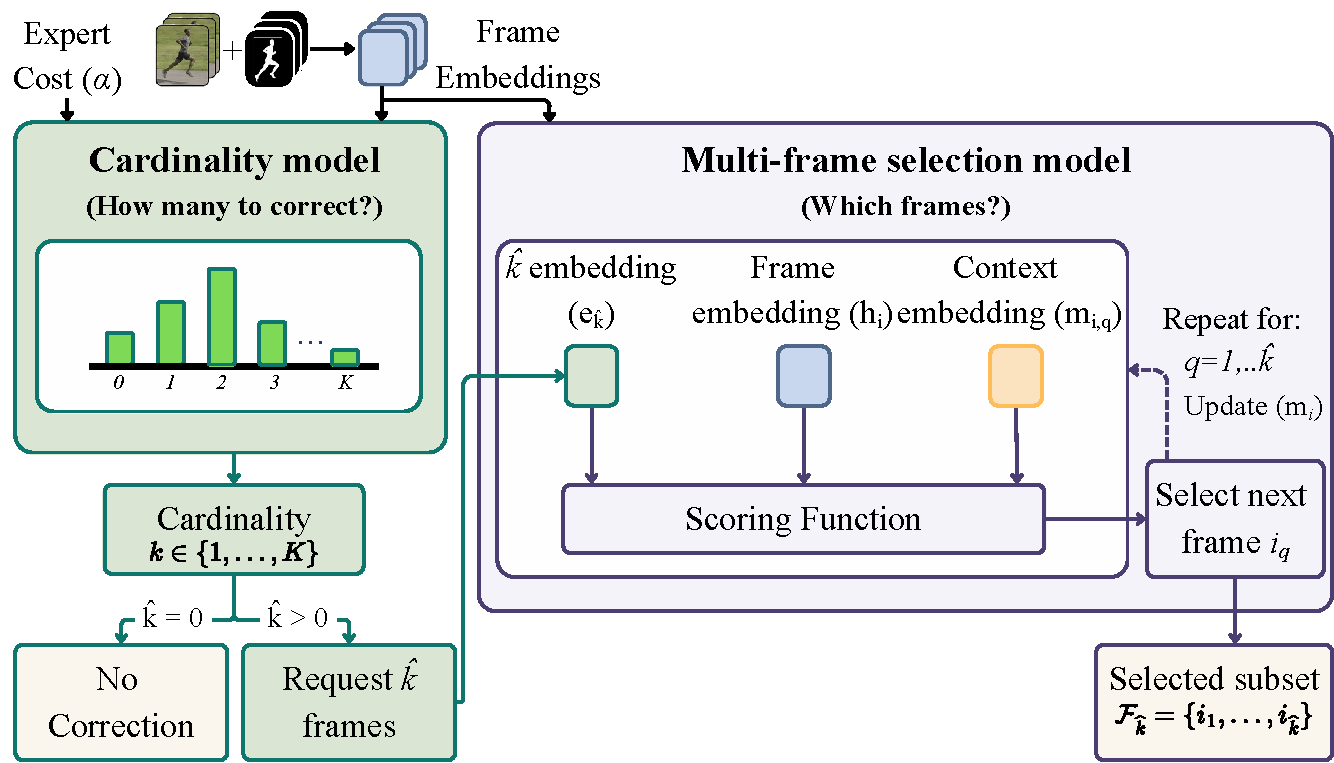
\includegraphics[width=\columnwidth]{Figures/architecture.pdf}
    \caption{
    Overview of the proposed cost-aware multi-frame deferral framework.
    Given the video frame embeddings and expert cost $\alpha$, the cardinality
    model predicts whether correction is required and, if so, the number of
    frames $\widehat{k}$ to prompt. Conditioned on the predicted cardinality, the
    multi-frame selection model constructs the correction set
    $\mathcal{F}_{\widehat{k}}=\{i_1,\ldots,i_{\widehat{k}}\}$ over
$\widehat{k}$ selection steps, updating the
    context after each selected frame. The resulting frames are then requested
    for expert prompting in a single correction round.
    }
    \label{fig:Architecture}
\end{figure}

\paragraph{Overview.}
A promptable video segmentation model requires an initial user prompt to
identify the object of interest. Given this required prompt, the segmentation
model propagates the corresponding object mask throughout the video to produce
an initial segmentation. Our framework evaluates this propagation to determine
whether additional corrective prompting is required, how many corrections
should be requested, and where they should be placed. As shown in
Figure~\ref{fig:Architecture}, the framework consists of two main components:
a cardinality model and a multi-frame selection model. The cardinality model
selects \(\widehat{k}\in\{0,\ldots,K\}\) by balancing the expected
segmentation improvement from additional corrections against their expert
prompting cost. If \(\widehat{k}=0\), the initial propagation is retained
because the expected improvement does not justify the expert cost. Otherwise,
the multi-frame selection model selects \(\widehat{k}\) frames for expert
annotation. The expert annotates all selected frames, and the segmentation
model uses the resulting prompts together to update the segmentation
throughout the video in a single propagation.

\subsection{Preliminaries}

\subsubsection{Learning-to-Defer.}

Conventional learning to defer considers a system composed of a machine
predictor and a human expert. Given an input \(x\), the machine produces a
prediction \(\widehat{y}^{m}\), while the expert can provide an alternative
prediction \(\widehat{y}^{e}\). A deferral policy
\(r(x)\in\{0,1\}\) decides whether to retain the machine prediction or
defer to the expert. Given the ground-truth target \(y\), the resulting
system loss is
\begin{equation}
\begin{aligned}
\mathcal{L}_{\mathrm{L2D}}(\mathsf{r},x,y)
={}&
\mathbf{1}\!\left[\mathsf{r}(x)=0\right]
\ell_m\!\left(y,\widehat{y}^{m}\right)
\\
&+
\mathbf{1}\!\left[\mathsf{r}(x)=1\right]
\left[
\ell_e\!\left(y,\widehat{y}^{e}\right)+\alpha
\right],
\end{aligned}
\label{eq:conventional_l2d}
\end{equation}
where \(\ell_m(\cdot)\) is the loss incurred when retaining the machine
prediction, \(\ell_e(\cdot)\) is the loss associated with the expert
prediction, and \(\alpha\) denotes the cost of requesting expert input.
The policy therefore learns to defer only when the expected reduction in
prediction loss justifies the additional expert cost.

\subsubsection{Promptable Video Segmentation Setting.}
\label{sec:expert_deferral_pvs}

In our setting of promptable video segmentation, the machine prediction is the segmentation
obtained by propagating an initial user prompt throughout a video. Expert
assistance does not replace this prediction directly; instead, the expert
provides corrective prompts on selected frames, which the segmentation model
uses to update the video-wide segmentation.

Formally, let \(v=(x_1,\ldots,x_N)\) denote a video containing \(N\)
frames, with corresponding ground-truth segmentation masks
\(y=(y_1,\ldots,y_N)\). For each frame \(i\), \(p_i\) denotes the
expert-provided annotation that serves as the user prompt to the segmentation
model. The set
\(\mathcal{F}_{\mathrm{init}}\subseteq\{1,\ldots,N\}\) contains the
indices of the initially prompted frames. These initial prompts identify the
object of interest and are required to initialise the promptable segmentation
model; they are therefore outside the corrective-prompting decision considered
by our framework.

Given the initial prompts, a promptable video segmentation model
\(s\) produces the initial propagated segmentation
\(
\widehat{y}
=
s\left(
v,
\{p_i\mid i\in\mathcal{F}_{\mathrm{init}}\}
\right).
\)
The propagation \(\widehat{y}\) plays the role of the machine prediction
in the learning-to-defer formulation. The set of unprompted frame indices
eligible for corrective prompting is
\(
\mathcal{E}
=
\{1,\ldots,N\}\setminus\mathcal{F}_{\mathrm{init}}.
\)

\subsection{Cost-aware multi-frame deferral}
\label{sec:cost_aware_multiframe_deferral}

Given the video \(v\) and its initial propagation \(\widehat{y}\), the
deferral policy determines whether corrective prompts are required and, if
so, how many should be requested. Let \(K\) denote the maximum number of
additional frame prompts that may be requested for a video, and assume that
\(\lvert\mathcal{E}\rvert\geq K\). The policy selects
\(
r(v,\widehat{y})\in\{0,\ldots,K\},
\)
where \(r(v,\widehat{y})=0\) retains the initial propagation and
\(r(v,\widehat{y})=k>0\) requests prompts on \(k\) additional frames.

For each \(k>0\), let
\(\mathcal{F}_k\subseteq\mathcal{E}\) denote the selected set of
correction-frame indices, where \(\lvert\mathcal{F}_k\rvert=k\). After
obtaining the corresponding expert prompts, the resulting segmentation is
\(
\widehat{y}_k
=
s\left(
v,
\{p_i\mid
i\in\mathcal{F}_{\mathrm{init}}\cup\mathcal{F}_k\}
\right).
\)

Let \(\ell(y,\widehat{y})\) denote the video-level segmentation loss.
The cost-aware multi-frame deferral objective is
\begin{equation}
\begin{aligned}
\mathcal{L}_{\mathrm{MF\text{-}L2D}}
={}&
\mathbf{1}[r(v,\widehat{y})=0]\,
\ell(y,\widehat{y})
\\
&+
\sum_{k=1}^{K}
\mathbf{1}[r(v,\widehat{y})=k]\,
\left[
\ell(y,\widehat{y}_k)+\alpha k
\right],
\end{aligned}
\label{eq:multi_frame_l2d}
\end{equation}
where \(\alpha\) is the cost of one additional expert prompt. For
\(k>0\), the reduction from
\(\ell(y,\widehat{y})\) to \(\ell(y,\widehat{y}_k)\) represents the
segmentation gain obtained from correction, while \(\alpha k\) represents
the corresponding expert cost.

We implement this decision using a cardinality model and a multi-frame
selection model. The cardinality model determines whether the initial
propagation should be retained or predicts the number of correction frames
to request. Given a positive cardinality, the multi-frame selection model
selects the corresponding frames from \(\mathcal{E}\).

\begin{table*}[t]
\caption{
Comparison of variable-cardinality deferral across four datasets at
\(\alpha=0.01\). We report segmentation quality
(\(\mathrm{mIoU}\uparrow\)), mean selected cardinality
(\(\widehat{k}\downarrow\)), and mean system cost
(\(c_{\widehat{k}}\downarrow\)), where
\(c_{\widehat{k}}=(1-\mathrm{mIoU})+\alpha\widehat{k}\).
Under \(\mathcal{K}\), \(\{0\}\), \(\{0,1\}\), and \(\{0{:}4\}\) denote
the allowed correction cardinalities. Rand., Single, Online, Indep., and
Multi. denote random-subset selection, single-frame selection, online
triggering, independent ranking, and multi-frame selection, respectively.
}
\label{tab:overall_comparison}

\centering
\small
\setlength{\tabcolsep}{2pt}
\renewcommand{\arraystretch}{1.0}
\begin{tabular}{@{}lcc|ccc|ccc|ccc|ccc@{}}
\toprule
& & & \multicolumn{3}{c|}{\textbf{VOST}} & \multicolumn{3}{c|}{\textbf{CAMotion}} & \multicolumn{3}{c|}{\textbf{SUN-SEG}} & \multicolumn{3}{c}{\textbf{VTUS}} \\
\textbf{Method} & $\boldsymbol{k}$ & \textbf{Sel.}
 & mIoU$\uparrow$ & $\hat{k}\!\downarrow$ & $c\!\downarrow$
 & mIoU$\uparrow$ & $\hat{k}\!\downarrow$ & $c\!\downarrow$
 & mIoU$\uparrow$ & $\hat{k}\!\downarrow$ & $c\!\downarrow$
 & mIoU$\uparrow$ & $\hat{k}\!\downarrow$ & $c\!\downarrow$ \\
\midrule
No correction & $0$ & -- & $.473$ & $0.00$ & $.527$ & $.802$ & $0.00$ & $.198$ & $.711$ & $0.00$ & $.289$ & $.627$ & $0.00$ & $.373$ \\
Random & $0{:}4$ & Rand. & $.587_{\pm.005}$ & $2.00$ & $.433$ & $.819_{\pm.003}$ & $2.00$ & $.201$ & $.762_{\pm.008}$ & $2.00$ & $.258$ & $.694_{\pm.004}$ & $2.00$ & $.326$ \\
L2RP~\cite{rasanjalee2026understanding} & $0{,}1$ & Single & $.602_{\pm.002}$ & $0.76$ & $.406$ & $.822_{\pm.002}$ & $0.47$ & $.183$ & $.774_{\pm.006}$ & $0.52$ & $.231$ & $.722_{\pm.001}$ & $0.88$ & $.287$ \\
Lazy-XMem~\cite{vujasinovic2024strike} & $0{:}4$ & Online & $.644$ & $3.33$ & $.390$ & $.845$ & $3.11$ & $.186$ & $.830$ & $3.65$ & $.207$ & $.764$ & $4.00$ & $.276$ \\
LECODU~\cite{zhang2024learning} & $0{:}4$ & Rand. & $.658_{\pm.001}$ & $3.21$ & $.374$ & $.837_{\pm.002}$ & $1.28$ & $.176$ & $.836_{\pm.004}$ & $2.01$ & $.184$ & $.755_{\pm.002}$ & $3.26$ & $.278$ \\
Top-$k(x)$~\cite{montreuil2025ask} & $0{:}4$ & Indep. & $.662_{\pm.005}$ & $2.82$ & $.366$ & $.838_{\pm.002}$ & $1.30$ & $.175$ & $.842_{\pm.005}$ & $1.80$ & $.176$ & $.795_{\pm.005}$ & $2.90$ & $.234$ \\
\textbf{Ours} & $\mathbf{0{:}4}$ & \textbf{Multi.} & $\mathbf{.699}_{\pm.002}$ & $2.56$ & $\mathbf{.327}$ & $\mathbf{.847}_{\pm.001}$ & $1.19$ & $\mathbf{.165}$ & $\mathbf{.850}_{\pm.003}$ & $1.71$ & $\mathbf{.167}$ & $\mathbf{.819}_{\pm.002}$ & $2.81$ & $\mathbf{.209}$ \\
\midrule
\textit{Oracle} & $\mathit{0{:}4}$ & \textit{Best} & $.714$ & $2.86$ & $.314$ & $.851$ & $1.10$ & $.160$ & $.874$ & $1.84$ & $.144$ & $.831$ & $2.87$ & $.198$ \\
\bottomrule
\end{tabular}

\end{table*}


\subsection{Cardinality model}
\label{sec:cardinality_model}

The cardinality model implements the deferral policy \(r\). Given the video
and its initial propagation, it outputs \(K+1\) scores and assigns a
probability
\(
\Pr_{\phi}(k\mid v,\widehat{y})
\)
to each action \(k\in\{0,\ldots,K\}\). The action \(k=0\) retains the
initial propagation, whereas \(k>0\) specifies the number of frames to be
selected by the multi-frame selection model.

At inference, the predicted cardinality is
\(
\widehat{k}
=
r(v,\widehat{y})
=
\arg\max_{k\in\{0,\ldots,K\}}
\Pr_{\phi}(k\mid v,\widehat{y}).
\)
If \(\widehat{k}=0\), no further expert prompt is requested. Otherwise,
the multi-frame selection model selects
\(\mathcal{F}_{\widehat{k}}\), and the expert annotations on these frames
are applied together to update the segmentation throughout the video.

\subsection{Multi-frame selection model}
\label{sec:multi_frame_selector}

For a specified cardinality \(k>0\), the multi-frame selection model selects
\(k\) frame indices from \(\mathcal{E}\) over \(q=1,\ldots,k\) selection
steps. This sequential process allows each decision to account for previously
selected frames, avoiding redundant choices without explicitly enumerating
every possible subset. The sequentiality is over the selected-set size rather
than video time, and all remaining eligible frames are considered at each step.

Throughout these selection steps, the segmentation remains
\(\widehat{y}\). Previously selected frames are added to the selection
context, but they are not yet annotated, and the segmentation model is not
re-propagated. Thus, all \(k\) frames are selected before their annotations
are requested from the expert.

An encoder produces a representation \(\mathbf{h}_i\) for every frame
\(i\in\{1,\ldots,N\}\) using the video frame \(x_i\) and its initially
propagated mask \(\widehat{y}_i\). At selection step \(q\), let
\(
\mathcal{F}_{q-1}
=
\{i_1,\ldots,i_{q-1}\}
\)
contain the frame indices selected at the preceding steps. The corresponding
context is
\(
\mathcal{C}_{q-1}
=
\mathcal{F}_{\mathrm{init}}\cup\mathcal{F}_{q-1}.
\)
At the first selection step (\(q=1\)),
\(\mathcal{F}_0=\varnothing\), and hence
\(\mathcal{C}_0=\mathcal{F}_{\mathrm{init}}\).
This context allows each candidate to be evaluated by the information it adds
to the frames already selected.

For each remaining candidate
\(i\in\mathcal{E}\setminus\mathcal{F}_{q-1}\), we apply soft cross-attention,
using the candidate representation as the query and the context-frame
representations as the keys and values. This produces a candidate-specific
context representation
\(
\mathbf{m}_{i,q}
=
\operatorname{attn}
\left(
\mathbf{h}_i,
\{\mathbf{h}_j\mid j\in\mathcal{C}_{q-1}\}
\right).
\)
Each supported cardinality \(k\) also has a learned embedding
\(\mathbf{e}_k\), allowing the scoring function to adapt its frame preferences
to the requested set size. The candidate score is
\(
z^{(k)}_{i,q}
=
\operatorname{score}_{\theta}
\left(
[\mathbf{h}_i;\mathbf{m}_{i,q};\mathbf{e}_k]
\right).
\)
The attention and scoring functions are shared across all candidates,
selection steps, and supported cardinalities.

The conditional probability of selecting candidate \(i\) at step \(q\) is
\(
\Pr_{\theta}
\left(
i_q=i
\mid
v,\widehat{y},\mathcal{C}_{q-1},k
\right)
=
\frac{
\exp\left(z^{(k)}_{i,q}\right)
}{
\displaystyle
\sum_{j\in\mathcal{E}\setminus\mathcal{F}_{q-1}}
\exp\left(z^{(k)}_{j,q}\right)
}.
\)
During training, \(i_q\) is drawn by categorical sampling from this
distribution. During inference, the candidate with the highest probability
is selected. The partial set is then updated as
\(
\mathcal{F}_q
=
\mathcal{F}_{q-1}\cup\{i_q\},
\)
and the context-dependent representations and candidate scores are
recalculated for the next step. The original frame representations
\(\{\mathbf{h}_i\}_{i=1}^{N}\) remain fixed throughout this process.

After \(k\) steps, the sequence
\(
\pi_k=(i_1,\ldots,i_k)
\)
records the selection order, while the final output is the frame-index set
\(
\mathcal{F}_k=\{i_1,\ldots,i_k\}\subseteq\mathcal{E}.
\)
The probability of the selection trajectory is
\begin{equation}
\Pr_{\theta}
\left(
\pi_k\mid v,\widehat{y},k
\right)
=
\prod_{q=1}^{k}
\Pr_{\theta}
\left(
i_q
\mid
v,\widehat{y},\mathcal{C}_{q-1},k
\right).
\label{eq:trajectory_probability}
\end{equation}
The sequence \(\pi_k\) is used to factorise the selection probability
during training; the final decision is the unordered frame set
\(\mathcal{F}_k\).

\subsection{Training objectives}
\label{sec:training_objectives}

\paragraph{Reward-Based Multi-Frame Selection.}
A video may contain multiple useful correction-frame sets, so the
multi-frame selection model is not trained to reproduce a single predefined
target set. Instead, it is trained using the segmentation loss obtained after
prompting the selected frames.

For each cardinality \(k\), we sample \(B\) alternative frame-index sets
\(\mathcal{R}_1,\ldots,\mathcal{R}_B\) from \(\mathcal{E}\), where
\(\lvert\mathcal{R}_b\rvert=k\) and
\(\mathcal{R}_b\neq\mathcal{F}_k\). Prompting the frames in
\(\mathcal{R}_b\) produces
\(
\widehat{y}_{\mathcal{R}_b}
=
s\left(
v,
\{p_i\mid
i\in\mathcal{F}_{\mathrm{init}}\cup\mathcal{R}_b\}
\right).
\)
The lowest segmentation loss among these sampled alternatives is
\(
b_k
=
\min_{1\leq b\leq B}
\ell\left(y,\widehat{y}_{\mathcal{R}_b}\right),
\)
and the advantage of the model-selected set is
\(
a_k
=
b_k-\ell(y,\widehat{y}_k).
\)
The frame-selection loss for cardinality \(k\) is
\begin{equation}
\mathcal{L}^{(k)}_{\mathrm{FS}}
=
-a_k
\log
\Pr_{\theta}
\left(
\pi_k\mid v,\widehat{y},k
\right).
\label{eq:frame_selection_loss}
\end{equation}
A positive advantage indicates that the selected set produces a lower
segmentation loss than the sampled alternatives and therefore increases its
selection probability. A negative advantage reduces its probability.

The multi-frame selection model is trained across all supported
cardinalities \(k\in\{1,\ldots,K\}\), with
\(
\mathcal{L}_{\mathrm{FS}}
=
\frac{1}{K}
\sum_{k=1}^{K}
\mathcal{L}^{(k)}_{\mathrm{FS}}.
\label{eq:frame_selection_total_loss}
\)
The frozen segmentation model is executed within the training loop to
generate the post-correction masks and rewards. For each cardinality, it
evaluates the selected set and $B$ sampled alternatives, requiring
$K(B+1)$ online propagations per video update without enumerating all
possible frame subsets.
\paragraph{Cost-Aware Cardinality Training.}
The multi-frame selection model is trained first and then frozen. During
cardinality-model training, the frozen selection model produces one frame
set \(\mathcal{F}_k\) for each supported cardinality \(k>0\). For every
cardinality \(k\in\{0,\ldots,K\}\), we compute the corresponding system cost
as
\begin{equation}
c_k=
\begin{cases}
\ell(y,\widehat{y}), & k=0,\\
\ell(y,\widehat{y}_k)+\alpha k, & k>0.
\end{cases}
\end{equation}
Thus, \(c_0\) is the system cost of retaining the initial propagation,
whereas \(c_k\) for \(k>0\) additionally includes the cost of requesting
\(k\) expert prompts. The cardinality targets therefore reflect the
trade-off between segmentation quality and expert effort.

To make the objective in Equation~\eqref{eq:multi_frame_l2d} trainable, we
adapt a cost-weighted multiclass surrogate loss \cite{cortes2024cardinalityawaresetpredictiontopk}. The action costs are
normalised independently for each video to obtain
\(\widetilde{c}_k\in[0,1]\), and the cardinality loss is
\begin{equation}
\mathcal{L}_{\mathrm{card}}
=
-
\sum_{k=0}^{K}
\left(1-\widetilde{c}_k\right)
\log
\Pr_{\phi}(k\mid v,\widehat{y}).
\label{eq:cardinality_loss}
\end{equation}
Actions with lower system cost receive larger weights, allowing the model to
learn the relative quality--cost trade-off among all supported cardinalities.

During cardinality model training, the frozen segmentation model evaluates one
selected set for each positive cardinality, requiring $K$ online
propagations per video update. Neither training stage enumerates the
combinatorial set of possible frame subsets. At inference, the cardinality
model predicts one $\widehat{k}$ and the selector chooses all
$\widehat{k}$ frames without intermediate segmentation reruns. Once their
expert prompts are available, SAM2 incorporates them through a single
corrected propagation.
